
\begin{QUOTE}{}{}
如何用 $\text{Splay}$ 维护二叉查找树。
\end{QUOTE}

\hr

\subsection{简介}

$\text{Splay}$ 是一种二叉查找树,它通过不断将某个节点旋转到根节点,使得整棵树仍然满足二叉查找树的性质,并且保持平衡而不至于退化为链,它由 Daniel Sleator 和 Robert Tarjan 发明。

\hr

\subsection{结构}

\subsubsection{二叉查找树的性质}

首先肯定是一棵二叉树!

能够在这棵树上查找某个值的性质:左儿子的值 $<$ 根节点的值 $<$ 右儿子的值。

\subsubsection{节点维护信息}

\begin{tabular}{lllllll}
\hline
rt& tot& fa[i]& ch[i][0/1]& val[i]& cnt[i]& sz[i]\\根节点编号& 节点个数& 父亲& 左右儿子编号& 节点权值& 权值出现次数& 子树大小\\\hline
\end{tabular}

\hr

\subsection{操作}

\subsubsection{基本操作}

\begin{itemize}
\item $\text{maintain}(x)$:在改变节点位置前,将节点 $x$ 的 $\text{size}$ 更新。
\item $\text{get}(x)$:判断节点 $x$ 是父亲节点的左儿子还是右儿子。
\item $\text{clear}(x)$:销毁节点 $x$。
\end{itemize}

\begin{cppcode}
void maintain(int x) { sz[x] = sz[ch[x][0]] + sz[ch[x][1]] + cnt[x]; }
bool get(int x) { return x == ch[fa[x]][1]; }
void clear(int x) { ch[x][0] = ch[x][1] = fa[x] = val[x] = sz[x] = cnt[x] = 0; }
\end{cppcode}

\subsubsection{旋转操作}

为了使 $\text{Splay}$ 保持平衡而进行旋转操作,旋转的本质是将某个节点上移一个位置。

\textbf{旋转需要保证}:

\begin{itemize}
\item 整棵 $\text{Splay}$ 的中序遍历不变(不能破坏二叉查找树的性质)。
\item 受影响的节点维护的信息依然正确有效。
\item $root$ 必须指向旋转后的根节点。
\end{itemize}

在 $\text{Splay}$ 中旋转分为两种:左旋和右旋。

\begin{figure}[htbp]
\centering
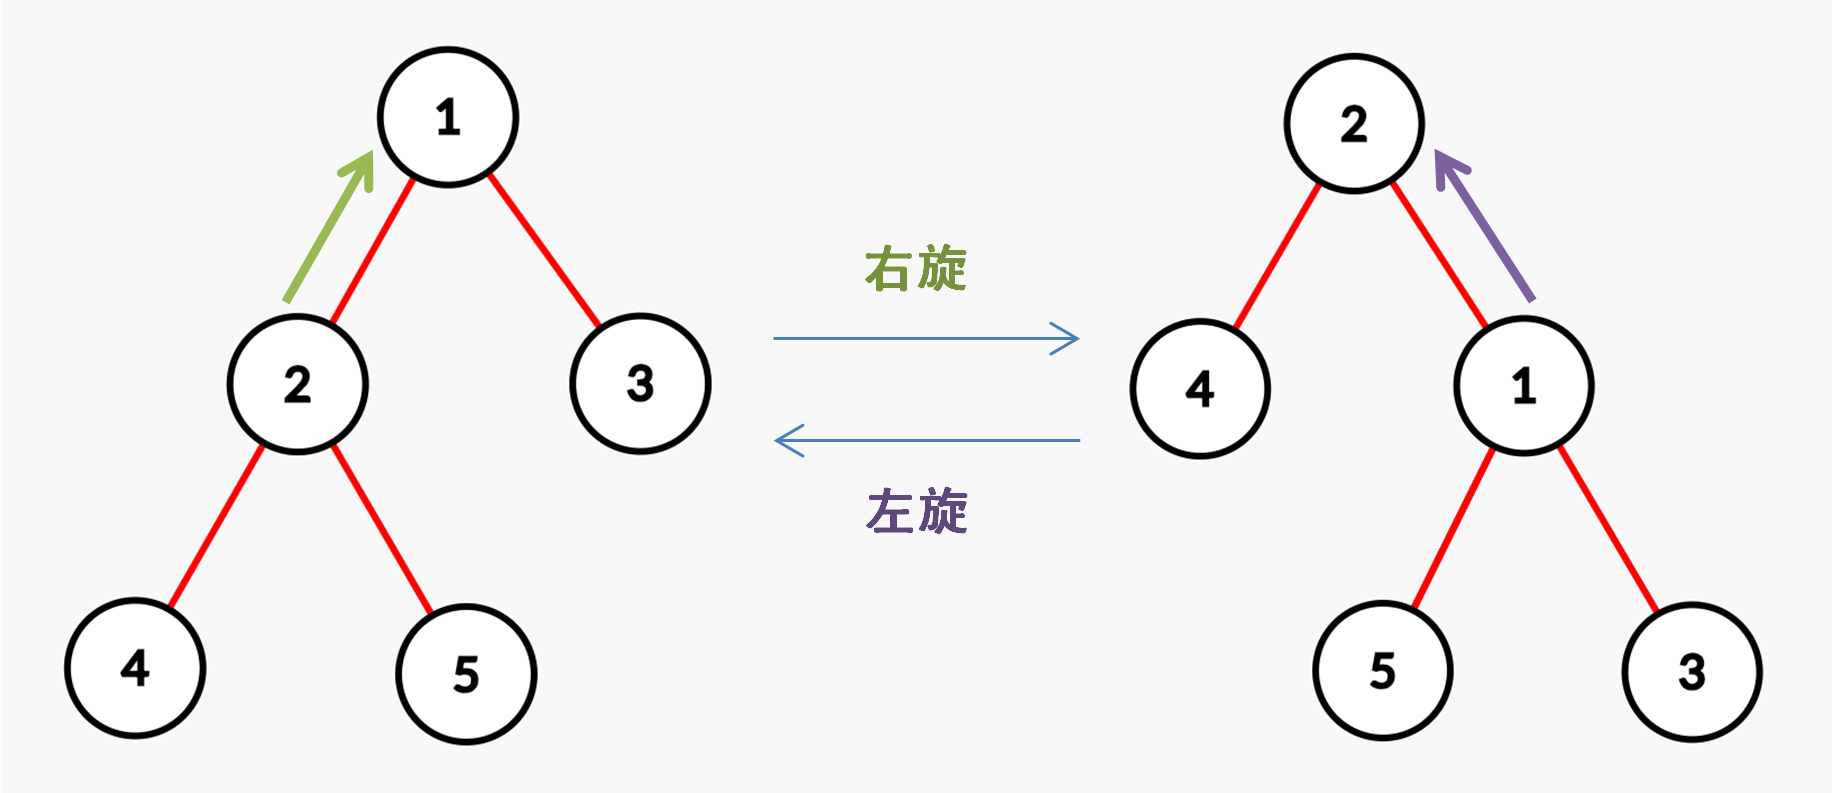
\includegraphics[width=0.7\textwidth]{docs/ds/images/splay2.png} 

\end{figure}

\textbf{具体分析旋转步骤}(假设需要旋转的节点为 $x$,其父亲为 $y$,以右旋为例)

\begin{enumerate}
\item 将 $y$ 的左儿子指向 $x$ 的右儿子,且 $x$ 的右儿子的父亲指向 $y$。
\texttt{ch[y][0]=ch[x][1]; fa[ch[x][1]]=y;}
\item 将 $x$ 的右儿子指向 $y$,且 $y$ 的父亲指向 $x$。
\texttt{ch[x][chk\textasciicircum{}1]=y; fa[y]=x;}
\item 如果原来的 $y$ 还有父亲 $z$,那么把 $z$ 的某个儿子(原来 $y$ 所在的儿子位置)指向 $x$,且 $x$ 的父亲指向 $z$。
\texttt{fa[x]=z; if(z) ch[z][y==ch[z][1]]=x;}
\end{enumerate}

\begin{cppcode}
void rotate(int x) {
  int y = fa[x], z = fa[y], chk = get(x);
  ch[y][chk] = ch[x][chk ^ 1];
  fa[ch[x][chk ^ 1]] = y;
  ch[x][chk ^ 1] = y;
  fa[y] = x;
  fa[x] = z;
  if (z) ch[z][y == ch[z][1]] = x;
  maintain(x);
  maintain(y);
}
\end{cppcode}

\subsubsection{Splay 操作}

$\text{Splay}$ 规定:每访问一个节点后都要强制将其旋转到根节点。此时旋转操作具体分为 $6$ 种情况讨论(其中 $x$ 为需要旋转到根的节点)

\begin{figure}[htbp]
\centering
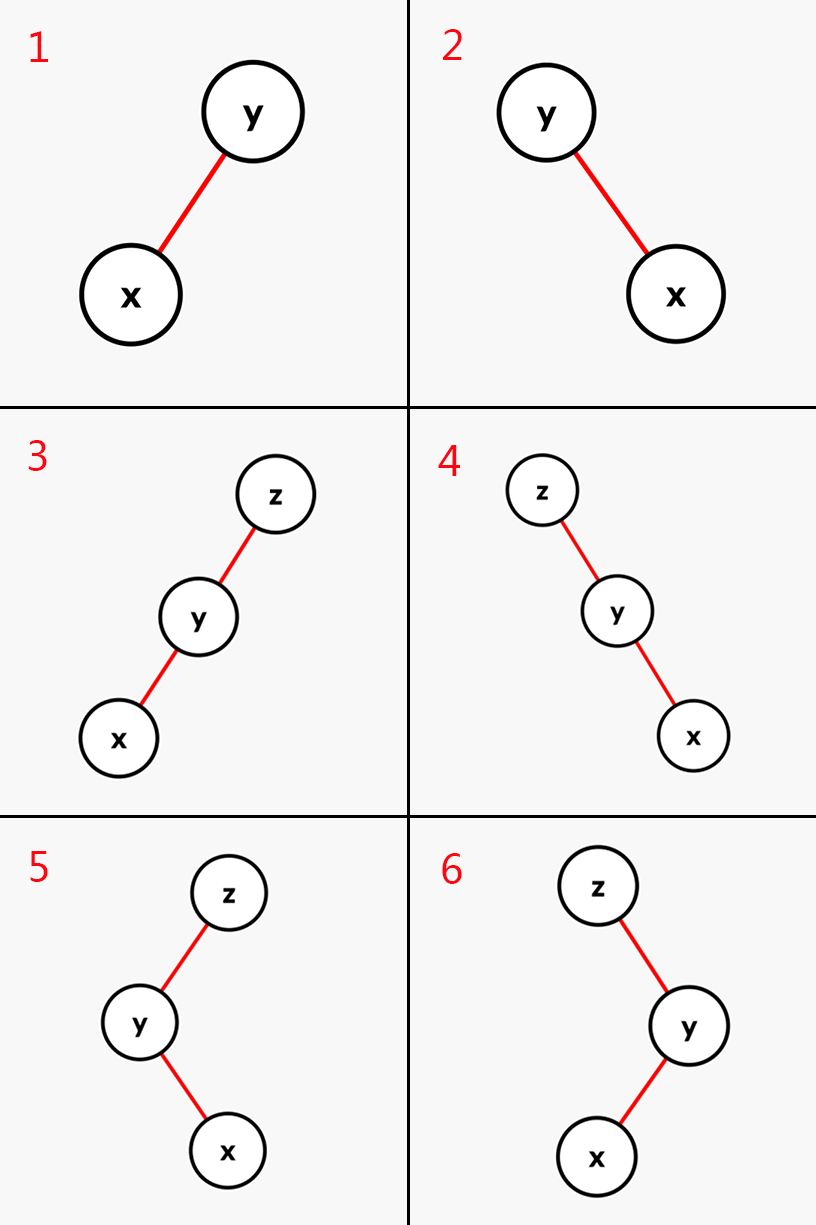
\includegraphics[width=0.7\textwidth]{docs/ds/images/splay1.png} 

\end{figure}

\begin{itemize}
\item 如果 $x$ 的父亲是根节点,直接将 $x$ 左旋或右旋(图 $1,2$)。
\item 如果 $x$ 的父亲不是根节点,且 $x$ 和父亲的儿子类型相同,首先将其父亲左旋或右旋,然后将 $x$ 右旋或左旋(图 $3,4$)。
\item 如果 $x$ 的父亲不是根节点,且 $x$ 和父亲的儿子类型不同,将 $x$ 左旋再右旋、或者右旋再左旋(图 $5,6$)。
\end{itemize}

分析起来一大串,其实代码一小段。大家可以自己模拟一下 $6$ 种旋转情况,就能理解 $\text{Splay}$ 的基本思想了。

\begin{cppcode}
void splay(int x) {
  for (int f = fa[x]; f = fa[x], f; rotate(x))
    if (fa[f]) rotate(get(x) == get(f) ? f : x);
  rt = x;
}
\end{cppcode}

\subsubsection{插入操作}

插入操作是一个比较复杂的过程,具体步骤如下(插入的值为 $k$):

\begin{itemize}
\item 如果树空了则直接插入根并退出。
\item 如果当前节点的权值等于 $k$ 则增加当前节点的大小并更新节点和父亲的信息,将当前节点进行 $\text{Splay}$ 操作。
\item 否则按照二叉查找树的性质向下找,找到空节点就插入即可(当然别忘了 $\text{Splay}$ 操作哦)。
\end{itemize}

\begin{cppcode}
void ins(int k) {
  if (!rt) {
    val[++tot] = k;
    cnt[tot]++;
    rt = tot;
    maintain(rt);
    return;
  }
  int cnr = rt, f = 0;
  while (1) {
    if (val[cnr] == k) {
      cnt[cnr]++;
      maintain(cnr);
      maintain(f);
      splay(cnr);
      break;
    }
    f = cnr;
    cnr = ch[cnr][val[cnr] < k];
    if (!cnr) {
      val[++tot] = k;
      cnt[tot]++;
      fa[tot] = f;
      ch[f][val[f] < k] = tot;
      maintain(tot);
      maintain(f);
      splay(tot);
      break;
    }
  }
}
\end{cppcode}

\subsubsection{查询 x 的排名}

根据二叉查找树的定义和性质,显然可以按照以下步骤查询 $x$ 的排名:

\begin{itemize}
\item 如果 $x$ 比当前节点的权值小,向其左子树查找。
\item 如果 $x$ 比当前节点的权值大,将答案加上左子树($size$)和当前节点($cnt$)的大小,向其右子树查找。
\item 如果 $x$ 与当前节点的权值相同,将答案加 $1$ 并返回。
\end{itemize}

注意最后需要进行 $\text{Splay}$ 操作。

\begin{cppcode}
int rk(int k) {
  int res = 0, cnr = rt;
  while (1) {
    if (k < val[cnr]) {
      cnr = ch[cnr][0];
    } else {
      res += sz[ch[cnr][0]];
      if (k == val[cnr]) {
        splay(cnr);
        return res + 1;
      }
      res += cnt[cnr];
      cnr = ch[cnr][1];
    }
  }
}
\end{cppcode}

\subsubsection{查询排名 x 的数}

设 $k$ 为剩余排名,具体步骤如下:

\begin{itemize}
\item 如果左子树非空且剩余排名 $k$ 不大于左子树的大小 $size$,那么向左子树查找。
\item 否则将 $k$ 减去左子树的和根的大小。如果此时 $k$ 的值小于等于 $0$,则返回根节点的权值,否则继续向右子树查找。
\end{itemize}

\begin{cppcode}
int kth(int k) {
  int cnr = rt;
  while (1) {
    if (ch[cnr][0] && k <= sz[ch[cnr][0]]) {
      cnr = ch[cnr][0];
    } else {
      k -= cnt[cnr] + sz[ch[cnr][0]];
      if (k <= 0) return val[cnr];
      cnr = ch[cnr][1];
    }
  }
}
\end{cppcode}

\subsubsection{查询前驱}

前驱定义为小于 $x$ 的最大的数,那么查询前驱可以转化为:将 $x$ 插入(此时 $x$ 已经在根的位置了),前驱即为 $x$ 的左子树中最右边的节点,最后将 $x$ 删除即可。

\begin{cppcode}
int pre() {
  int cnr = ch[rt][0];
  while (ch[cnr][1]) cnr = ch[cnr][1];
  return cnr;
}
\end{cppcode}

\subsubsection{查询后继}

后继定义为大于 $x$ 的最小的数,查询方法和前驱类似:$x$ 的右子树中最左边的节点。

\begin{cppcode}
int nxt() {
  int cnr = ch[rt][1];
  while (ch[cnr][0]) cnr = ch[cnr][0];
  return cnr;
}
\end{cppcode}

\subsubsection{删除操作}

删除操作也是一个比较复杂的操作,具体步骤如下:

\begin{itemize}
\item 首先将 $x$ 旋转到根的位置。
\item 接下来分为多个情况考虑:
\end{itemize}

\begin{enumerate}
\item 如果有不止一个 $x$,那么将 $cnt[x]$ 减 $1$ 并退出。
\item 如果 $x$ 没有儿子节点,那么直接将当前节点 $\text{clear}$ 并退出。
\item 如果 $x$ 只有一个儿子,那么先将当前节点 $\text{clear}$ 再把唯一的儿子作为根节点。
\item 否则将 $x$ 的前驱旋转到根并作为根节点,将 $x$ 的右子树接到根节点的右子树上,最后要将根的信息更新。
\end{enumerate}

\begin{cppcode}
void del(int k) {
  rk(k);
  if (cnt[rt] > 1) {
    cnt[rt]--;
    maintain(rt);
    return;
  }
  if (!ch[rt][0] && !ch[rt][1]) {
    clear(rt);
    rt = 0;
    return;
  }
  if (!ch[rt][0]) {
    int cnr = rt;
    rt = ch[rt][1];
    fa[rt] = 0;
    clear(cnr);
    return;
  }
  if (!ch[rt][1]) {
    int cnr = rt;
    rt = ch[rt][0];
    fa[rt] = 0;
    clear(cnr);
    return;
  }
  int x = pre(), cnr = rt;
  splay(x);
  fa[ch[cnr][1]] = x;
  ch[x][1] = ch[cnr][1];
  clear(cnr);
  maintain(rt);
}
\end{cppcode}

\hr

\subsection{完整代码}

\begin{cppcode}
#include <cstdio>
const int N = 100005;
int rt, tot, fa[N], ch[N][2], val[N], cnt[N], sz[N];
struct Splay {
  void maintain(int x) { sz[x] = sz[ch[x][0]] + sz[ch[x][1]] + cnt[x]; }
  bool get(int x) { return x == ch[fa[x]][1]; }
  void clear(int x) {
    ch[x][0] = ch[x][1] = fa[x] = val[x] = sz[x] = cnt[x] = 0;
  }
  void rotate(int x) {
    int y = fa[x], z = fa[y], chk = get(x);
    ch[y][chk] = ch[x][chk ^ 1];
    fa[ch[x][chk ^ 1]] = y;
    ch[x][chk ^ 1] = y;
    fa[y] = x;
    fa[x] = z;
    if (z) ch[z][y == ch[z][1]] = x;
    maintain(x);
    maintain(y);
  }
  void splay(int x) {
    for (int f = fa[x]; f = fa[x], f; rotate(x))
      if (fa[f]) rotate(get(x) == get(f) ? f : x);
    rt = x;
  }
  void ins(int k) {
    if (!rt) {
      val[++tot] = k;
      cnt[tot]++;
      rt = tot;
      maintain(rt);
      return;
    }
    int cnr = rt, f = 0;
    while (1) {
      if (val[cnr] == k) {
        cnt[cnr]++;
        maintain(cnr);
        maintain(f);
        splay(cnr);
        break;
      }
      f = cnr;
      cnr = ch[cnr][val[cnr] < k];
      if (!cnr) {
        val[++tot] = k;
        cnt[tot]++;
        fa[tot] = f;
        ch[f][val[f] < k] = tot;
        maintain(tot);
        maintain(f);
        splay(tot);
        break;
      }
    }
  }
  int rk(int k) {
    int res = 0, cnr = rt;
    while (1) {
      if (k < val[cnr]) {
        cnr = ch[cnr][0];
      } else {
        res += sz[ch[cnr][0]];
        if (k == val[cnr]) {
          splay(cnr);
          return res + 1;
        }
        res += cnt[cnr];
        cnr = ch[cnr][1];
      }
    }
  }
  int kth(int k) {
    int cnr = rt;
    while (1) {
      if (ch[cnr][0] && k <= sz[ch[cnr][0]]) {
        cnr = ch[cnr][0];
      } else {
        k -= cnt[cnr] + sz[ch[cnr][0]];
        if (k <= 0) return val[cnr];
        cnr = ch[cnr][1];
      }
    }
  }
  int pre() {
    int cnr = ch[rt][0];
    while (ch[cnr][1]) cnr = ch[cnr][1];
    return cnr;
  }
  int nxt() {
    int cnr = ch[rt][1];
    while (ch[cnr][0]) cnr = ch[cnr][0];
    return cnr;
  }
  void del(int k) {
    rk(k);
    if (cnt[rt] > 1) {
      cnt[rt]--;
      maintain(rt);
      return;
    }
    if (!ch[rt][0] && !ch[rt][1]) {
      clear(rt);
      rt = 0;
      return;
    }
    if (!ch[rt][0]) {
      int cnr = rt;
      rt = ch[rt][1];
      fa[rt] = 0;
      clear(cnr);
      return;
    }
    if (!ch[rt][1]) {
      int cnr = rt;
      rt = ch[rt][0];
      fa[rt] = 0;
      clear(cnr);
      return;
    }
    int x = pre(), cnr = rt;
    splay(x);
    fa[ch[cnr][1]] = x;
    ch[x][1] = ch[cnr][1];
    clear(cnr);
    maintain(rt);
  }
} tree;

int main() {
  int n, opt, x;
  for (scanf("%d", &n); n; --n) {
    scanf("%d%d", &opt, &x);
    if (opt == 1)
      tree.ins(x);
    else if (opt == 2)
      tree.del(x);
    else if (opt == 3)
      printf("%d\n", tree.rk(x));
    else if (opt == 4)
      printf("%d\n", tree.kth(x));
    else if (opt == 5)
      tree.ins(x), printf("%d\n", val[tree.pre()]), tree.del(x);
    else
      tree.ins(x), printf("%d\n", val[tree.nxt()]), tree.del(x);
  }
  return 0;
}
\end{cppcode}

\hr

\section{例题}

以下题目都是裸的 $\text{Splay}$ 维护二叉查找树。\sout{(直接套板子即可)}

\begin{itemize}
\item \href{https://www.luogu.org/problemnew/show/P3369}{【模板】普通平衡树}
\item \href{https://www.lydsy.com/JudgeOnline/problem.php?id=1588}{HNOI2002 营业额统计}
\item \href{https://www.lydsy.com/JudgeOnline/problem.php?id=1208}{HNOI2004 宠物收养所}
\end{itemize}

\section{练习题}

\href{https://www.lydsy.com/JudgeOnline/problem.php?id=1552}{bzoj 1552 Cerc2007 robotic sort} (权限题)

\href{https://www.luogu.org/problemnew/show/P3380}{luogu P3380 【模板】二逼平衡树(树套树)}

\href{https://www.lydsy.com/JudgeOnline/problem.php?id=2827}{bzoj 2827 千山鸟飞绝}

\href{https://www.lydsy.com/JudgeOnline/problem.php?id=4923}{bzoj 4923 Lydsy1706 月赛K 小值查询}

\hr

\begin{QUOTE}{}{}
本文部分内容引用于 \href{https://algocode.net}{algocode 算法博客},特别鸣谢!
\end{QUOTE}
